%-------------------------------------------------------------------------------
%-------------------------------------------------------------------------------
\begin{frame}\begin{center}
	\LARGE\textbf{Model}
\end{center}\end{frame}
%-------------------------------------------------------------------------------
%-------------------------------------------------------------------------------
\begin{frame}
	\textbf{Generalized Roy model}
	\begin{align*}\begin{array}{l@{\qquad}l}
			\text{Potential Outcomes} &\text{Observed Outcome}\\
			Y_1 = \mu_1(X) + U_1      &  Y = D Y_1 + (1 - D)Y_0 \\
			Y_0 = \mu_0(X) + U_0      &\\
			& \\
			\text{Choice} & \\
			D = \mathrm{I}[\mu_D(X, Z) - V > 0] & \\
		\end{array}
	\end{align*}

\end{frame}

\begin{frame}\begin{center}
		\LARGE\textit{Individual Heterogeneity}
\end{center}\end{frame}
%-------------------------------------------------------------------------------
%-------------------------------------------------------------------------------
\begin{frame}
	Individual-specific Benefit of Treatment
	\begin{align*}
		Y_1 - Y_0 = (\mu_1(X) - \mu_0(X)) + (U_1 - U_0)\\
	\end{align*}
	\textbf{Sources of Heterogeneity}
	\begin{itemize}\setlength\itemsep{1em}
		\item Difference in observables
		\item Difference in unobservables\medskip
		\begin{itemize}\setlength\itemsep{1em}
			\item Uncertainty
			\item Private information
		\end{itemize}
	\end{itemize}
\end{frame}
%-------------------------------------------------------------------------------
%-------------------------------------------------------------------------------
\begin{frame}
\begin{figure}[htp]\centering\caption{Distribution of benefits}
\scalebox{0.35}{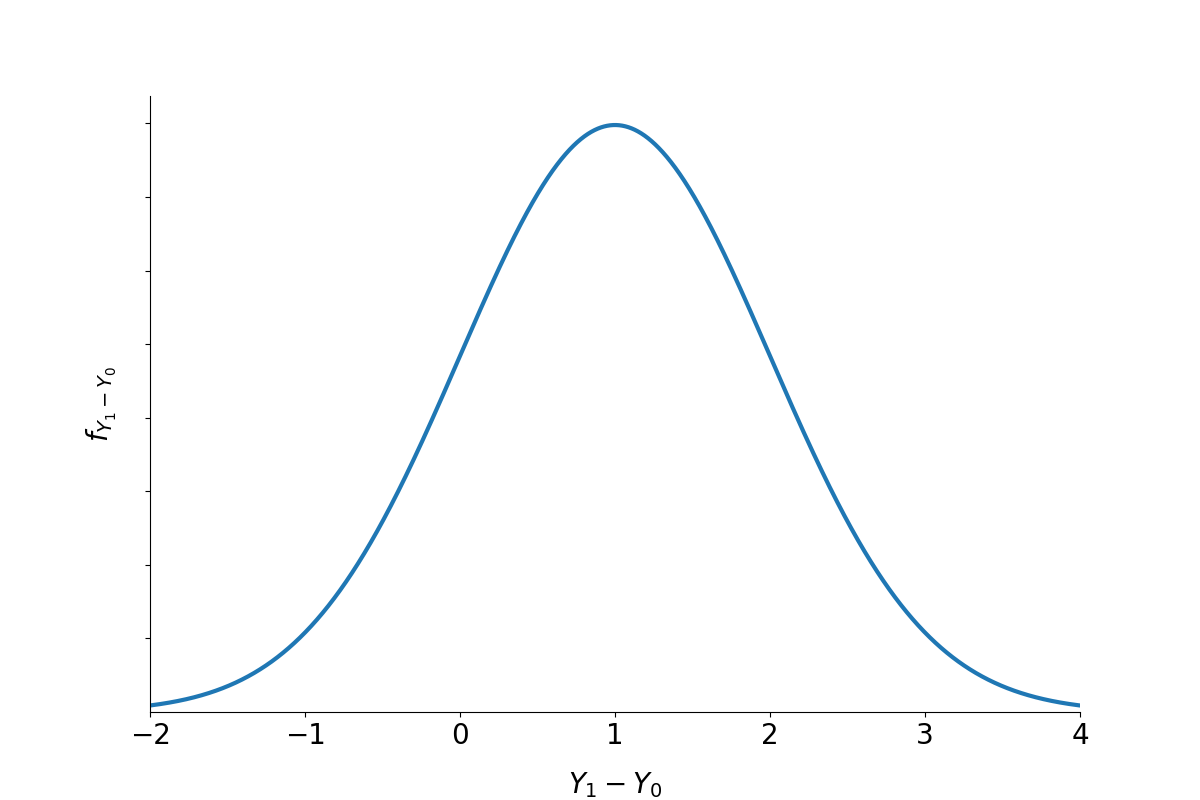
\includegraphics{fig-treatment-effects-benefits}}
\end{figure}
\end{frame}
%-------------------------------------------------------------------------------
%-------------------------------------------------------------------------------
\begin{frame}\textbf{Econometric problems}

\begin{itemize}\setlength\itemsep{1em}
\item \textbf{Evaluation problem}, we only observe an individual in either the treated or untreated state.
\item \textbf{Selection problem}, individuals that select into treatment differ from those that do not.
\end{itemize}

\end{frame}
%-------------------------------------------------------------------------------
%-------------------------------------------------------------------------------
\begin{frame}
	\textbf{Essential Heterogeneity}\\\vspace{0.5cm}
	\textbf{Definition:} Individuals select their treatment status based on
	gains unobservable by the econometrician. More formally,
	\begin{align*}
		Y_1 - Y_0 \notindep D\quad \mid X = x.
	\end{align*}
	\(\Rightarrow\) consequences for the choice of the estimation strategy
\end{frame}
%-------------------------------------------------------------------------------
%-------------------------------------------------------------------------------
